%!TEX root = batch-course.tex
\begin{frame}\frametitle{DuPont Nylon example: learning from new data}

	\begin{itemize}
		\item	Industrial data set of \( N = 55 \) batches from Nylon production
		
		\item	Temperature, pressure and flow rate variables: \( K = 10\)  batch tags
		
		\item	Batch duration about 2 hours (\( J=100 \) time intervals)
		
		\item	12 hours before lab values returned: batch-to-batch adjustment not possible
		
		\item	Known problems with batches: 40, 41, 42, 50, 51, 53, 54, 55
	\end{itemize}
	
	
\end{frame}

\begin{frame}\frametitle{DuPont Nylon example: raw data}
	{\color{myGreen}{Note}}: data were scaled for confidentiality
	\begin{center}
		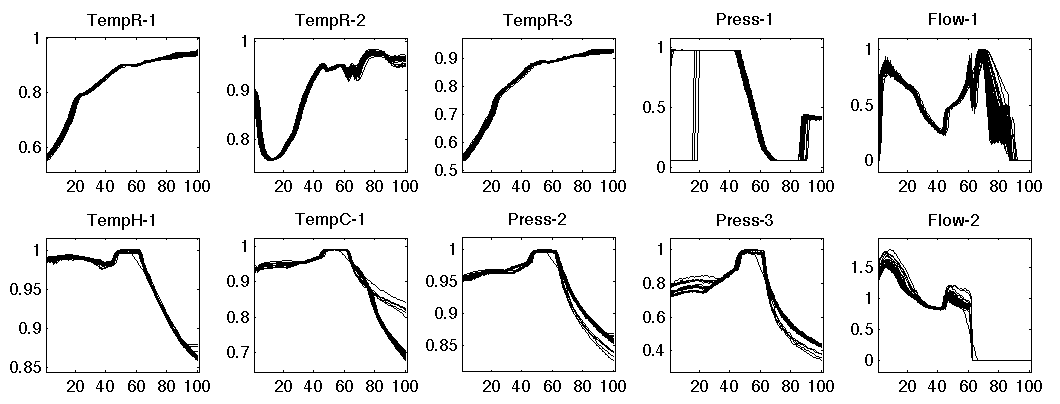
\includegraphics[width=\textwidth]{images/dupont/dupont-raw-data-trajectories.png}
	\end{center}
	
	\vspace{1cm}
	\begin{itemize}
		\item	Can see a few unusual batches: see ``Temp-C1'' and ``Press-1'' tags
		
		\item	Alignment looks pretty good (process is well controlled)
		
		\item	Some periods are noisy: ``Flow-1'' and ``Flow-2''
	\end{itemize}
\end{frame}

\begin{frame}\frametitle{DuPont Nylon example: initial PCA}
	\begin{itemize}

		\item	Just start with 2 components initially
		
				\begin{itemize}					
					\item	no cross-validation, just get a ``feel'' for the data
					\item	\( R^2_X = [38.28\%, 17.58\%]\), or cumulatively: 55.9\%
				\end{itemize}
		
		\item	Score plot:
				
				\begin{columns}
					\column{0.8\textwidth}
						\begin{center}
							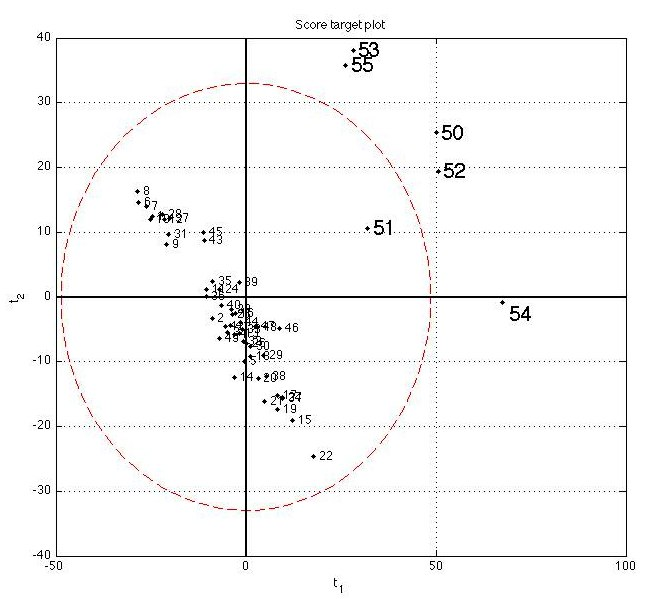
\includegraphics[width=0.8\textwidth]{images/dupont/dupont-raw-score-plot.jpg}
							% batch_PCA = lvm({'X', batch_X}, 2);
							% plot(batch_PCA, 'scores', {'labels'})
						\end{center}
						
					\column{0.4\textwidth}
						\begin{itemize}
							\item	Batches 50 to 55 unusual
							
							\item	Distorted the model		
							
							\item	Before excluding them and rebuilding model, let's first examine them.
						\end{itemize}
				\end{columns}
	\end{itemize}
\end{frame}

\begin{frame}\frametitle{DuPont Nylon example: initial PCA}
	\begin{itemize}
		\item	SPE plot
	\end{itemize}
	
	\begin{center}
		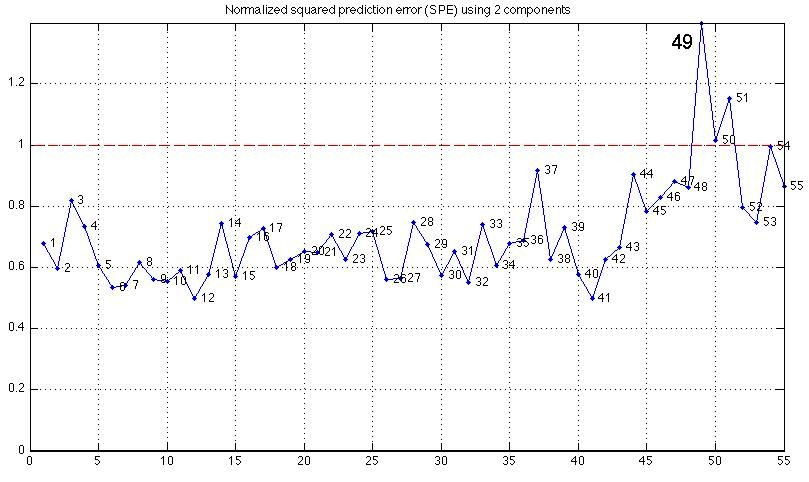
\includegraphics[width=\textwidth]{images/dupont/dupont-raw-SPE.jpg}
		% batch_PCA = lvm({'X', batch_X}, 2);
		% plot(batch_PCA, 'spe', {'labels'})
	\end{center}
\end{frame}

\begin{frame}\frametitle{DuPont Nylon example: batch 54 (high \( t_1 \) batch)}
	\begin{itemize}
		\item	Contribution plot in \( t_1 \)
	\end{itemize}
	
	\begin{center}
	\end{center}
\end{frame}

\begin{frame}\frametitle{DuPont Nylon example: Summary}
	
\begin{enumerate}
	\item	Plot the trajectories
	
			\begin{itemize}
				\item	Sometime outlier batches already detectable
				
				\item	Visualize how good your alignment is: do data need extra pretreatment?
			\end{itemize}
\end{enumerate}


	
\end{frame}

